\graphicspath{{capitulos/Capitulo2-Definicion-del-problema/recursos/}}

\section{Definición del problema} \label{apartado:2}

Tal y como se ha introducido antes, el proyecto ABACO pretende automatizar el proceso de creación de un horario de trabajo para
los distintos controladores del espacio aéreo de forma que dada una sectorización de este, todos los sectores puedan ser
controlados siguiendo las pautas establecidas por el dominio del problema.

El control del espacio aéreo (también conocido como ATC, \textit{Air Trafic Control}) es una tarea que se lleva a cabo en todos los aeropuertos con el fin de monitorizar los diferentes aviones que sobrevuelan una determinada zona del cielo, de cara a garantizar la seguridad de sus rutas (lo que se denomina control de ruta), así como de sus aterrizajes (que se llama control de aproximación o de área terminal), encargándose también de las comunicaciones de voz tanto tierra-aire con los pilotos de las aeronaves (vía radio), como tierra-tierra con otros controladores u otro personal de gestión (vía telefónica) \cite{ENAIRE-web, wazir2013mobile}.
La zona de trabajo de los controladores aéreos se denomina Centros de Control de Tráfico Aéreo.

\subsection{Sectores y sectorización}
En primera lugar, explicaremos brevemente cómo se divide el espacio aéreo del territorio español, cuyo organismo encargado de su gestión es ENAIRE
\footnote{\url{https://www.enaire.es/sobre_enaire/conoce_enaire/quienes_somos_ENAIRE}}. 
Si bien la realidad es muy compleja, aquí unicamente describiremos una simplificación de la misma, omitiéndose detalles técnicos de aviación que no son necesarios para la implementación del sistema.
\\

El espacio aéreo mundial se encuentra dividido en \textit{FIR}s (\textit{Flight Information Region}), áreas del territorio sobre las que se mueven los diferentes aviones de cada compañía aérea de cada país, en la \refcruzada{Figura}{fig:fireuropa} puede verse gráficamente los límites de cada región. En el caso de España, podemos ver que tiene control sobre 3 \textit{FIR}s: el de Barcelona, el de Madrid y el de Canarias, sin embargo, a nivel nacional, existen algunas subdivisiones denominadas \textit{Dependencias} (ya que dependen del \textit{FIR} en el que se encuentren), que permiten una mejor gestión del territorio:
\begin{itemize}
	\item Barcelona RutaE
	\item Barcelona RutaW
	\item Barcelona TMA ESTE
	\item Barcelona TMA NORTE
	\item Barcelona TMA OESTE
	\item Canarias ACC App
	\item Canarias ACC Ruta
	\item Madrid Ruta 1
	\item Madrid Ruta 2
	\item Madrid TMA NORTE
	\item Madrid TMA SUR
	\item Malaga App
	\item Palma TACC
	\item Sevilla TACC
	\item  Valencia TACC TMA
\end{itemize}

Algunos de ellos aparecerán en los casos reales de prueba del sistema, que pueden verse en el \refcruzada{Apartado}{apartado:5}
\begin{figure}
	\centering
	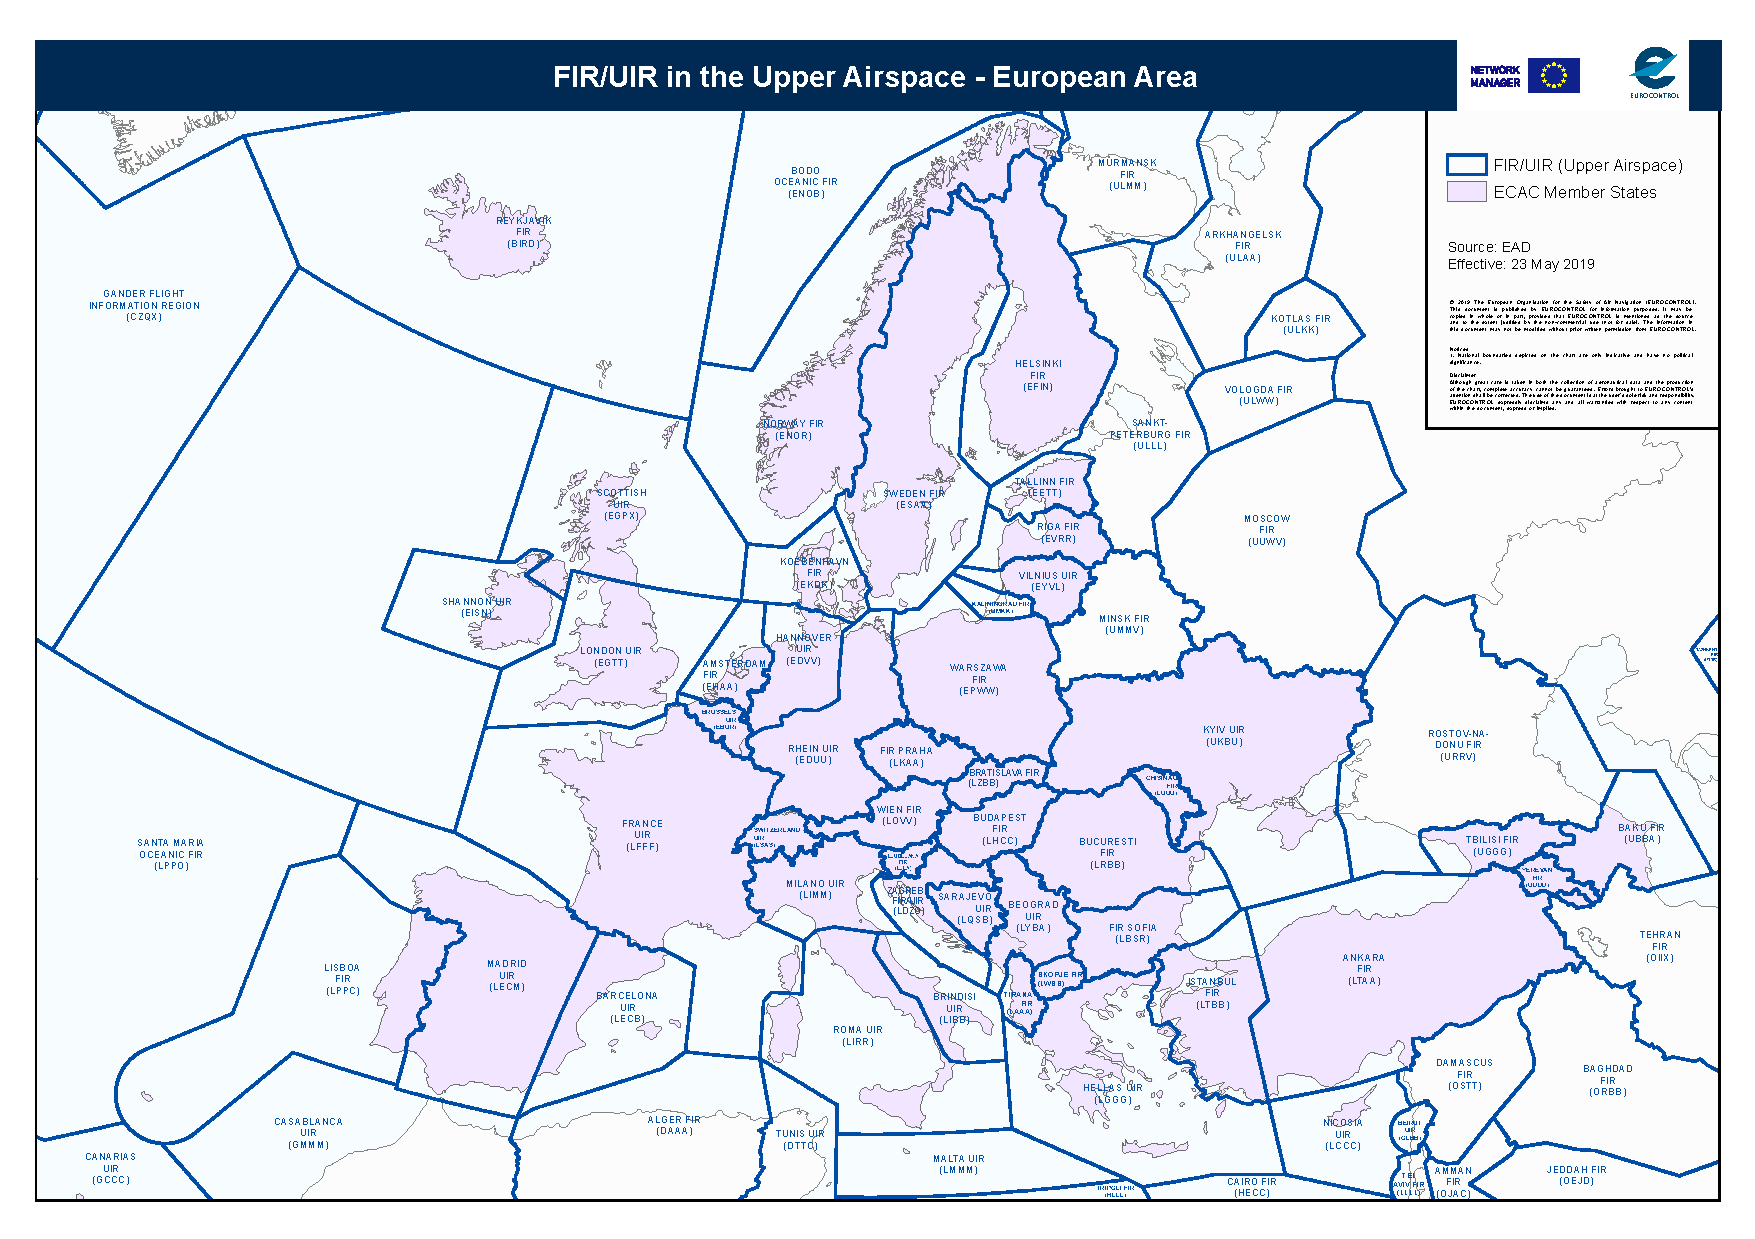
\includegraphics[width=1\linewidth]{FIR_europa}
	\caption{FIRs del la zona europea. Fuente: EUROCONTROL}
	\label{fig:fireuropa}
\end{figure}


